\documentclass[10pt,a4paper]{article}
\usepackage[UTF8,fontset = windows]{ctex}
\setCJKmainfont[BoldFont=黑体,ItalicFont=楷体]{等线}
\usepackage{amssymb,amsmath,amsfonts,amsthm,mathrsfs,dsfont,graphicx}
\usepackage{ifthen,indentfirst,enumerate,color,titletoc}
\usepackage{tikz}
\usetikzlibrary{arrows,calc,intersections,patterns}
\usepackage[bf,small,indentafter,pagestyles]{titlesec}
\usepackage[top=1in, bottom=1in,left=0.8in,right=0.8in]{geometry}
\renewcommand{\baselinestretch}{1.65}
\newtheorem{defi}{定义~}
\newtheorem{eg}{例~}
\newtheorem{ex}{~}
\newtheorem{rem}{注~}
\newtheorem{thm}{定理~}
\newtheorem{coro}{推论~}
\newtheorem{axiom}{公理~}
\newtheorem{prop}{性质~}
\newcommand{\blank}[1]{\underline{\hbox to #1pt{}}}
\newcommand{\bracket}[1]{(\hbox to #1pt{})}
\newcommand{\onech}[4]{\par\begin{tabular}{p{.9\textwidth}}
A.~#1\\
B.~#2\\
C.~#3\\
D.~#4
\end{tabular}}
\newcommand{\twoch}[4]{\par\begin{tabular}{p{.46\textwidth}p{.46\textwidth}}
A.~#1& B.~#2\\
C.~#3& D.~#4
\end{tabular}}
\newcommand{\vartwoch}[4]{\par\begin{tabular}{p{.46\textwidth}p{.46\textwidth}}
(1)~#1& (2)~#2\\
(3)~#3& (4)~#4
\end{tabular}}
\newcommand{\fourch}[4]{\par\begin{tabular}{p{.23\textwidth}p{.23\textwidth}p{.23\textwidth}p{.23\textwidth}}
A.~#1 &B.~#2& C.~#3& D.~#4
\end{tabular}}
\newcommand{\varfourch}[4]{\par\begin{tabular}{p{.23\textwidth}p{.23\textwidth}p{.23\textwidth}p{.23\textwidth}}
(1)~#1 &(2)~#2& (3)~#3& (4)~#4
\end{tabular}}
\begin{document}
\begin{enumerate}[1.]
% 第一讲 8+3+7
\item 用适当符号($\in$,$\notin$,$=$,$\subsetneq$)填空:$\pi$\blank{10}$\mathbf{Q}$; $\{x|x=2k+1, \ k\in \mathbf{Z}\}$\blank{10}$\{x|x=2k-1,k\in \mathbf{Z}\}$; $\{3.14\}$\blank{10}$\mathbf{Q}$; $\{y|y=x^2\}$\blank{10}$\{x|y=x^2\}$.  
\item 已知$P=\{y=x^2+1\}$, $Q=\{y|y=x^2+1, \ x\in \mathbf{R}\}$, $E=\{x|y=x^2+1, \  x\in \mathbf{R}\}$, $F=\{(x,y)|y=x^2+1, \ x\in \mathbf{R}\}$, $G=\{x|x\ge 1\}$, $H=\{x|x^2+1=0, \ x\in \mathbf{R}\}$, 则各集合间关系正确的有\blank{50}. (答案可能不唯一)\\
(A) $P=F$   (B) $Q=E$   (C) $E=F$   (D) $Q\subseteq G$  (E) $H\subsetneq P$
\item 设全集是实数集$\mathbf{R}$, $M=\{x|-2 \le x\le 2\}$, $N=\{x|x<1\}$, 则$\complement_U M\cap N=$\blank{50}.
\item 设$A=\{x|-4<x<4, \ x\in \mathbf{R}\}$, $B=(-\infty,1]\cup [3,+\infty)$, 则$\{x|x\in A, \ x\notin A\cap B  \}$=\blank{50}.
\item 设$A=\{x|x=\sqrt k, \ k\in \mathbf{N}\}$,$B=\{x|x\le 3,\ x\in \mathbf{Q}\}$, 则$A\cap B=$\blank{50}.
\item 设全集$U=\{2,3,a^2+2a-3\}$, 集合$A=\{|2a-1|,2\}$, $\complement_U A=\{5\}$, 则实数$a=$\blank{50}.
\item (1) 设$M=\{y|y=x^2, x\in \mathbf{R}\}$, $N=\{x|x=t,\ t\in \mathbf{R}\}$, 则$M\cap N=$\blank{50}.\\
(2) 设$M=\{(x,y)|y=x^2,\ x\in \mathbf{R}\}$, $N=\{(t,x)|x=t,\ t\in \mathbf{R}\}$, 则$M\cap N=$\blank{50}.
\item 设全集$U=\{1,2,3,4\}$, $\complement_U A\cap B=\{3\}$, $A\cap \complement_U B=\{2\}$, $\complement_U A\cup \complement_U B=\{2,3,4\}$, 则$\complement_U A\cap \complement_U B$=\blank{50}.
\item 集合$C=\{x|x=\dfrac k2\pm \dfrac14, \ k\in \mathbf{Z}\},D=\{x|x=\dfrac k4,\ k\in \mathbf{Z}\}$, 试判断$C$与$D$的关系, 并证明.
\item 集合$A=\{x|x^2+4x=0\}$, $B=\{x|x^2+2(a+1)x+a^2-1=0,\ x\in \mathbf{R}\}$.\\
(1) 若$A\cap B=A$, 求实数$a$的取值范围;\\
(2) 若$A\cup B=A$, 求实数$a$的取值范围.
\item 若集合$A=[2,3]$, 集合$B=[a,2a+1]$.\\
(1) 若$A\subsetneq B$, 求实数$a$的取值范围;\\
(2) 若$A\cap B\ne \varnothing$, 求实数$a$的取值范围.
\item 设全集$U=\mathbf{R}$, 集合$A=\{x|f(x)=0\}$, $B=\{x|g(x)=0\}$, $C=\{x|h(x)=0, \ x\in \mathbf{R}\}$, 则方程$\dfrac{f^2(x)+g^2(x)}{h(x)}=0$的解集是\blank{50}(用$U,A,B,C$表示).
\item (1) 已知集合$A=\{y|y=x^2, \ x\in \mathbf{R}\}, B=\{y|y=4-x^2, \ x\in \mathbf{R}\}$, 则$A\cap B=$\blank{50}.\\
(2) 已知集合$A=\{(x,y)|y={x^2},\ x\in \mathbf{R}\}$, $B=\{(x,y)|y=4-x^2, \ x\in \mathbf{R}\}$, 则$A\cap B=$\blank{50}.
\item 设$m\in \mathbf{R}$, 已知$A=\{x|x^2-3x+2=0\}$, $B=\{x|mx+1=0\}$, 且$B\subsetneq A$, 则$m=$\blank{50}.
\item (1) 集合$A$满足$\{1\}\subseteq A \subsetneq \{1,2,3,4\}$, 则满足条件的集合$A$有\blank{50}个.
(2) 若$A\cup B=\{1,2\}$, 将满足条件的集合$A$, $B$写成有序集合对$(A,B)$, 则有序集合对$(A,B)$有\blank{50}个.
\item 已知$A=\{x|x^2-3x+2=0\}$, $B=\{x|x^2-ax+a=0, \ x\in \mathbf{R}\}$, 若$B\subsetneq A$, 求满足题意的实数$a$.
\item 设集合$A=\{x|x^2+px+1=0,\ x\in \mathbf{R}\}$, 若$A\cap \mathbf{R}^+=\varnothing$. 求实数p的取值范围.
\item 设函数$f(x)=\lg (\dfrac2{x+1}-1)$的定义域为集合$A$, 函数$g(x)=\sqrt{1-|x+a|}$的定义域为集合$B$.\\
(1) 当$a=1$时, 求集合$B$.\\
(2) 问: $a\ge 2$是$A\cap B=\varnothing$的什么条件(在``充分非必要条件、必要非充分条件、充要条件、既非充分也非必要条件''中选一)?并证明你的结论.

% 第二讲 8+3+10

\item 如图, $U$为全集, $M,P,S$是$U$的三个子集, 则阴影部分所表示的集合是\bracket{20}.
\fourch{$(M\cap P)\cap S$}{$(M\cap P)\cup S$}{$(M\cap P)\cap \complement_U S$}{$(M\cap P)\cup \complement_U S$}
\begin{center}
    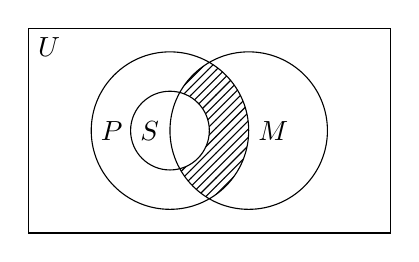
\begin{tikzpicture}
        \begin{scope}
            \clip (1,0) circle (1);
            \begin{scope}[even odd rule]
                \clip (0,0) circle (1) (0,0) circle (0.5);
                \filldraw [pattern = {north east lines}] (-2,-2) rectangle (2,2);
            \end{scope}
        \end{scope}
        \draw (0,0) circle (1) (1,0) circle (1) (0,0) circle (0.5);
        \draw (-1.8,-1.3) rectangle (2.8,1.3);
        \draw (-1.8,1.3) node [below right] {$U$} (-1,0) node [right] {$P$} (-0.5,0) node [right] {$S$} (1,0) node [right] {$M$};
    \end{tikzpicture}
\end{center}
\item 设集合$A=\{5,\log_2(a+3)\}$, $B=\{a,b\}$, 若$A\cap B=\{2\}$, 则$A\cup B=$\blank{50}.
\item 设集合$A\cap \{-2,0,1\}=\{0,1\}$, $A\cup \{-2,0,2\}=\{-2,0,1,2\}$, 则满足上述条件的集合$A$的个数为\blank{50}个.
\item 若集合$A=\{x|x\le 2\}$, $B=\{x|x\ge a\}$, 满足$A\cap B=\{2\}$, 则实数$a=$\blank{50}.
\item 若集合$M=[a-1,a+1]$, $N=(-\infty,-1)\cup [2,+\infty)$, 且$M\cap N=\varnothing$, 则实数$a$的取值范围为\blank{50}.
\item 集合$A=\{(x,y)|x^2+y^2=25\}$, $B=\{(x,y)|x=3y=4\}$, 则$A\cap B$的子集个数是\blank{50}个.
\item 已知集合$M=\{x|x=3m+1, \ m\in \mathbf{Z}\}$, $N=\{y|y=3m+2, \ m\in \mathbf{Z}\}$, 若$x_0\in M$, $y_0\in N$, 则$x_0y_0$与集合$M,N$的关系是\bracket{20}.
\twoch{$x_0y_0\in M$但$x_0y_0$$\notin N$}{$x_0y_0\in N$但$x_0y_0\notin M$}{$x_0y_0\notin M$且$x_0y_0\notin N$}{$x_0y_0$$\in M$且$x_0y_0\in N$}
\item 若$A=\{x|x=2n,\ n\in \mathbf{Z}\}$, $B=\{x|x=4m,\ m\in \mathbf{Z}\}$, 求证:$B\subsetneq A$.
\item 设常数$a\in \mathbf{R}$, 集合$A=\{x|\dfrac{3-2x}{x-1}+1 \ge 0, \ x\in \mathbf{R}\}$, $B=\{x|2ax<a+x, \ x\in \mathbf{R} \}$.若$A\cup B=B$, 求$a$的取值范围.
\item 设常数$m\in \mathbf{R}$, $A=\{(x,y)|x^2+mx-y+2=0,\ x\in \mathbf{R}\}$, $B=\{(x,y)|x-y+1=0, x\in M\}$, 且$A\cap B\ne\varnothing$.\\
(1) 若$M=\mathbf{R}$, 求实数$m$的取值范围;\\
(2) 若$M=(\dfrac13,2]$, 求实数$m$的取值范围.
\item 设常数$k\in \mathbf{R}$, 关于$x$的不等式组$\begin{cases} x^2-x-2>0, \\ 2x^2+(2k+5)x+5k<0 \end{cases}$ 整数解的集合为$\{-2\}$, 求实数$k$的取值范围.
\item 设$A=\{(x,y)|y=-4x+6,\ x\in \mathbf{R}\}, B=\{(x,y)|y=5x-3,\ x\in \mathbf{R}\}$, 则$A\cap B=$\blank{50}.
\item 已知$M=\{a|\dfrac6{5-a}\in \mathbf{N}, \ a\in \mathbf{Z}\}$, 则用列举法表示$M=$\blank{50}.
\item 定义集合运算: $A\odot B=\{z|z=xy(x+y), \ x\in A, \ y\in B \}$, 设集合$A=\{0,1\}$, $B=\{2,3\}$, 则集合$A\odot B$的所有元素之和为\blank{50}.
\item 已知全集$U=\mathbf{R}$, $A=\{-1\}$, $B=\{x|\lg (x^2-2)=\lg x\}$, 则\bracket{20}
\fourch{$A\subseteq B$}{$A\cup B=\varnothing$}{$A\supseteq B$}{$(\complement_U A)\cap B=\{2\}$}
\item 集合$A=\{(x,y)|y=|x|+1\}$, $B=\{(x,y)|y=\dfrac12x+a\}$, 若$A\cap B=\varnothing$, 则$a$的取值范围是\blank{50}.
\item 调查某班$50$名学生, 音乐爱好者有$40$人, 体育爱好者有$24$人, 则两方面都爱好的人数最少\blank{50}人, 最多\blank{50}人.
\item 已知集合$A=\{x|ax^2-3x+2=0\}$至多有一个元素, 则$a$的取值范围是\blank{50}; 若至少有一个元素, 则$a$的取值范围是\blank{50}.
\item 设含有三个实数的集合既可以表示为$\{a,\dfrac ba,1\}$, 又可以表示为$\{a^2,a+b,0\}$, 那么$a+b=$\blank{50}.
\item 设$f(x)=x^2-12x+36$, $A=\{a|1\le a\le 10, \ a\in \mathbf{N}\}$, $B=\{b|b=f(a),\ a\in A\}$, 又设$C=A\cap B$. 求集合$C$.
\item 设常数$m\in \mathbf{R}$, $A=\{(x,y)|y=-x^2+mx-1,\ x\in \mathbf{R}\}$, $B=\{(x,y)|x+y=3,\ x\in M\}$, 且$A\cap B$的子集有两个.\\
(1) 若$M=\mathbf{R}$, 求实数$m$的值;\\
(2) 若$M=[0,3]$, 求实数$m$的取值范围.

% 第三讲 8+3+8

\item 填写下列命题的否定形式:\\
(1) $m\le 0$或$n>0$: \blank{200};\\
(2) 空间三条直线$l,m,n$两两相交: \blank{200};\\
(3) 复数$z_1,z_2,z_3$中至多一个为纯虚数: \blank{200}.
\item 已知$a,b$是整数, 写出命题``若$ab$为偶数, 则$a+b$为偶数''的逆命题、否命题、逆否命题, 并判断所写命题的真假.\\
逆命题:\blank{200}, 真假: \blank{20};\\
否命题:\blank{200}, 真假: \blank{20};\\
逆否命题:\blank{200}, 真假: \blank{20}.
\item 设甲是乙的充分非必要条件, 乙是丙的充要条件, 丁是丙的必要非充分条件, 则丁是甲的() 
\twoch{充分非必要条件}{必要非充分条件}{充要条件}{既非充分又非必要条件}
\item 若$A$是$B$的必要非充分条件, 则$\overline{A}$是$\overline{B}$的\blank{50}条件.  
\item 下列各组命题中互为等价命题的是\bracket{20}.
\twoch{$A\subseteq B$与$A\cup B=B$}{$x\in A$且$x\in B$与$x\in A\cup B$}{$a\in A\cap B$与$a\in A$或$a\in B$}{$m\in A\cap B$与$m\in A\cup B$}
\item 填空(在``充分不必要''、``必要不充分''、``充要''、``既不充分也不必要''中选一种作答):\\
(1) ``$\alpha \ne \beta$''是$\cos \alpha \ne \cos \beta$''的\blank{50}条件;\\
(2) 在$\triangle ABC$中, ``$A=B$''是``$\sin A=\sin B$''的\blank{50}条件.
\item ``$a>0b>0$''的一个必要非充分条件是\bracket{20}.
\fourch{$a>0$}{$b>0$}{$a>0b>0$}{$a,b\in \mathbf{R}$}
\item ``函数$f(x)\ (x\in \mathbf{R})$存在反函数''是``函数$f(x)$在$\mathbf{R}$上为增函数''的\bracket{20}.
\twoch{充分而不必要条件}{必要而不充分条件}{充分必要条件}{既不充分也不必要条件}
\item 填空: (填``充分不必要''、``必要不充分''、``充要''、``既不充分也不必要'')\\ 
(1) 对于实数$x,y$, $p$: $xy>1$且$x+y>2$是$q$: $x>1$且$y>1$的\blank{50}条件;\\
(2) 对于实数$x,y$, $p$: $x+y\ne 8$是$q$: $x\ne 2$或$y\ne 6$的\blank{50}条件;\\
(3) 已知$x,y\in \mathbf{R}$, $p$: $(x-1)^2+(y-2)^2=0$是$q$: $(x-1)(y-2)=0$的\blank{50}条件;\\
*(4) 设$x,y\in \mathbf{R}$, 则``$x^2+y^2<2$''是``$|x|+|y|\le \sqrt2$''的\blank{50}条件; 又是``$|x|+|y|<2$''的\blank{50}条件; 又是``$|x|<\sqrt2$且$|y|<\sqrt2$''的\blank{50}条件.\\
(5) 设$a_1,b_1,c_1,a_2,b_2,c_2$均为非零实数, 方程$a_1x^2+b_1x+c_1=0$和方程$a_2x^2+b_2x+c_2=0$的实数解集分别为$M$和$N$, 则``$\dfrac{a_1}{a_2}=\dfrac{b_1}{b_2}=\dfrac{c_1}{c_2}$''是``$M=N$''的\blank{50}条件.
\item (1) 是否存在实数$m$, 使得$2x+m<0$是${x^2}-2x-3>0$的充分条件? 说明理由.\\
(2) 是否存在实数$m$, 使得$2x+m<0$是$x^2-2x-3>0$的必要条件? 说明理由.
\item 已知关于$x$的实系数二次方程$a x^2 +bx+c=0\ (a>0)$, 分别求下列命题的一个充要条件:\\
(1) 方程有一正根, 一根是零;\\
(2) 两根都比$2$小.
\item 设$a,b\in \mathbf{R}$, 写出命题``若$a+b>0$且$ab>0$, 则$a>0$且$b>0$''的逆否命题.
\item 填空(填``充分不必要''、``必要不充分''、``充要''、``既不充分也不必要''):\\
(1) 若$x,y\in \mathbf{R}$, 则$x^2+y^2 \ne 0$是``$x,y$不全为零''的\blank{50}条件;\\
(2) 若$x,y$$\in \mathbf{R}$, 则``$xy>0,x+y>0$''是``$x>0,y>0$'' 的\blank{50}条件;\\
(3) 设$a,b\in \mathbf{R}$, 则``$|a|+|b|=|a+b|$''是``$ab=0$''的\blank{50}条件;\\   
(4) 若$a,b,c$是常数, 则``$a>0$且$b^2-4ac<0$''是``对任意$x\in \mathbf{R}$, 有$ax^2+bx+c>0$''的\blank{50}条件;\\
(5) 设$a,b\in \mathbf{R},$则$b=\tan a$是$a=\arctan b$的\blank{50}条件.
\item 已知$x,y\in \mathbf{R}$, 有如下四个命题: \textcircled{1} $x^2+y^2<1$; \textcircled{2} $|x|+|y|<1$; \textcircled{3} $|x|<1$且$y|<1$; \textcircled{4} $|x+y|<1$. 则\blank{50}是\blank{50}的充分非必要条件(答案可能不唯一).
\item 使不等式$2x^2-5x-3\ge 0$成立的一个充分不必要条件是\bracket{20}. 
\fourch{$x<0$}{$x\ge 0$}{$x\in \{-1,3,5\}$}{$x\le \dfrac12$或x$\ge 3$}
\item 已知$\alpha$:``$x\ge a$'', $\beta$:``$|x-1|\le 1$'', 若$\alpha$是$\beta$的必要非充分条件, 则实数$a$的取值范围是\blank{50}.
\item 命题甲: 关于$x$的方程$x^2+x+m=0$有两个相异的负根; 命题乙: 关于$x$的方程$4x^2+x+m=0$无实根, 若这两个命题有且只有一个是真命题, 求实数$m$的取值范围.
*\item 已知$P=\{x|x^2-8x-20 \le 0\}$, $S=\{x||x-a|\le m\}$, 求实数$a,m$的值, 使得``$x\in P$''是``$x\in S$''的充要条件.
*\item 设$f(x)=ax^2+x+a$, 写出一个$a$的值,\\
(1) 使$f(x)>0\ (x\in \mathbf{R})$恒成立;\\
(2) 使$f(x)>0\ (x\in \mathbf{R})$恒不成立;\\
(3) 使$f(x)>0\ (x\in \mathbf{R})$不恒成立. 










 


\end{enumerate}

\end{document}